\chapter{\library{Lantern}: Data-driven Acoustic Echo Retrieval}\label{ch:lantern}

\marginpar{%
    \footnotesize
    \textbf{Keywords:} Acoustic Echo Retrieval, TDOA Estimation, Supervised Learning, Deep Learning, Robust Regression.
    \\\textbf{Resources:}
    \begin{itemize}
        \item \href{https://ieeexplore.ieee.org/document/8683534}{ICASSP2018 Paper}
        \item \href{https://github.com/Chutlhu/MIRAGE}{Code}
        \item \href{https://sigport.org/documents/mirage-2d-sound-source-localization-using-microphone-pair-augmentation-echoes}{ICASSP2018 Poster}
    \end{itemize}
}
\newthought{Synopsis} \synopsisChLantern

\mynewline
This chapter is structured in two sections: one devotes to present a quick overview deep learning model and how to train them, and one discusses their application to echo estimation.
The material concerning the first section are a personal digestion of material available in standard machine learning text book, such as~\citeonly{bishop2006pattern,goodfellow2016deep},
and audio related ones~\citeonly{vincent2018audio,muller2015fundamentals}.
We mention the recent comprehensive work of~\citeonly{purwins2019deep} on deep learning for general audio signal processing.
In the second section present part of the previously published work~\cite{di2019mirage} and of a technical report~\cite{di2019honda}.

\section{Introduction}
Recently \acfp{DNN} have capture the attention of many research field, due to recent advances that allow for faster implementation and training, and considerable performance improvement.
Therefore, \acp{DNN}s have been widely used in many domains.
They belong to the class of \textit{supervised} learning or \textit{data-driven} models, where the training step is performed on labeled data, namely input-output pairs.
The inclusion of these models in audio signal processing tasks has meant a considerable improvement in the performance, in particular audio and music source separation, speech enhancement, source localization (see  the related sections in~\cref{ch:application}).
\\Moreover, respect to traditional machine learning methods, the use of deep learning models presents other advantages.
They are flexible and adaptable across tasks; for instance, \acf{CNN}-based models from Computer Vision can be adapted for audio source separation (\eg/,~\citeonly{xiao2016deep, sainath2017multichannel, perotin2018crnn}), and for source localization(\eg/, ~\citeonly{chakrabarty2017broadband,vesperini2018localizing,nguyen2018autonomous,salvati2018exploiting}).
Furthermore, \acp{DNN}s reduce --- even remove --- the step of designing hand-crafted feature, by including the feature learning as part of the learning process.
\\Other
\marginpar{
    \itshape\footnotesize
    As part of a first investigation in this thesis work, the \acf{GLLiM} framework was considered for echo estimation.
    In fact, this thesis initially as a natural following up of the work~\citeonly{gaultier2017vast}.
    Then, we oriented our attention towards \ac{DNN} models which gave already satisfactory results.
    The highly non-linear nature of the mapping between echoes' properties and acoustic features which collides with the locally-linear assumption behind \ac{GLLiM}.
    Nevertheless, we recognize other benefits of the \ac{GLLiM} framework which cannot be found in \ac{DNN}-based approach.
    For instance, the ability of considering input missing data or including prior statistical information in the model.
} supervised learning methods have been proposed in the literature of audio processing, such as \ac{GMM}-based frameworks~\citeonly{laufer2013relative,deleforge2015acoustic,gaultier2017vast}.
This frameworks allows to build power models based on probabilistic prior knowledge and are compete with \ac{DNN} models in case of small training dataset.
However they ofter require strong assumption of the nature of the mapping between input-output pairs, such as (local-)linearity or independency between the variables.

\mynewline
The use of supervised learning models (not only the \ac{DNN}), presents some disadvantages.
One of the most relevant ones is their dependence on annotated data.
This is important bottleneck in audio signal processing task, because collecting and annotating comprehensive real-wold acoustic data is not trivial, since it requires proper tools, expertise and time.
In order to overcome this issue, a standard approach nowadays is to used training data generated by acoustic simulators.
We will refer to this approach as \textit{virtually supervised learning} and it provides a great versatility, for instance:
\begin{itemize}
    \item many different acoustic condition can be include in the training data,\\\eg/, different \acf{RT$_{60}$} and \acf{SNR} levels;
    \item a precise (up to computer precision) annotation of the data come directly,\\\eg/ spatial, temporal information of the audio scene events;
    \item and finally, the data can be potentially re-used for different application,\\\eg/, localization, separation, diarization, \etc/;
\end{itemize}
Therefore, the simulators provide a direct mapping for the parameters of interest to synthetic observations, which learning-based models aim to invert.
Besides, the solutions obtained in a data-driven fashion suffer from bias depending on the dataset used and may not be able to generalize to real-world scenario.
Interestingly, the work in~\citeonly{nguyen2018autonomous} discusses an automatic approach for collecting, annotating data automatically as a pre-calibration step.
However, this approach is possible only with certain technology (the authors programmed a humanoid robot equipped with a binaural hearing system that build a training set automatically).

\mynewline
The following sections gives a quick overview of relevant models used in our work with the intention of motivating the use for echo estimation.
The review includes basic theory behind neural networks and deep learning, optimization and loss functions, as well as the aspects related to training on
acoustic simulators.

\section{Deep Learning Model}

\subsection{Multi-layer perceptions}\label{subsec:lantern:mlp}
\acf{MLP} are simple and basic modules of \ac{DNN} and are also known as \textit{fully-connected} or \textit{dense layers}.
They consist of a sequence of layer, each of which defined by an affine transformation followed by a non-linearity function:
\begin{equation*}
    \bfy = f(\bfW \bfx + \bfb)
    ,
\end{equation*}
where
\newcommand{\Din}{\ensuremath{D_{\text{in}}}}
\newcommand{\Dout}{\ensuremath{D_{\text{out}}}}
\begin{itemize}
    \item $\bfx\in\bbR^{\Din}$ is the input,
    \item $\bfy\in\bbR^{\Dout}$ is the output,
    \item and $\bfb\in\bbR^{\Dout}$ and $\bfW\in\bbR^{\Dout \times \Din}$ are the \textit{bias vector} and the \textit{weight matrix}, respectively.
\end{itemize}
The function $f(\cdot)$ is a non-linear \textit{activation} function, which allows the model to learn non-linear structures.
Models built with these layers are typically used to map input to a representation space where problems (\eg/, classification and regression) can be addressed more easily.
The main drawback of these simple models is that are not invariant to scaled or shifted input.
Since in audio data, gain, temporal and frequency variations are common, they not suitable.
Nevertheless, \acp{MLP} are used in combination with other type of layers, such as \acfp{CNN}, \acfp{RNN}.

\newthought{Non-linear activation functions} are one of the key feature of \acp{DNN}.
Thanks to these, the model are able to achieve more \textit{expressive power} with respect to linear models~\citeonly{goodfellow2016deep}.
Without these functions, it can be shown that composition of affine transformations, is equivalent to a single affine transformation.
Therefore, the activation functions make the model capable to accounts for more complex relationships between the input and the output than an affine transformation.
Typical examples of these function are, for instance, hyperbolic tangent, the Sigmoid function, and \acf{ReLU}.

\subsection{Convolutional neural networks}\label{subsec:lantern:cnn}
The \ac{CNN} consists in convolutional layers that have been introduced to overcome some limitations of the simple linear ones.
In a nutshell, the consists of learnable kernel functions that are convolved with their input.
Therefore, they are characterized by
\begin{itemize}
    \item shift-invariance property, and can be used to reduce the model complexity since the same kernel can be used at different input location;
    \item the ability to detect local structures at different level of abstraction in the network (see~\cref{fig:lantern:features}).
\end{itemize}
Using a Python-like notation, a 2D-dimensional convolutional layer is defined by the following equation:
\begin{equation*}
    \bfY[:,:,k] = f( \sum_{i=0}^{I-1} \bfW[:,:,i,k] \convDis \bfX[:,:,i] + \bfb[:,:,k])
    ,
\end{equation*}
where
\begin{itemize}
    \item $\bfX_k\in\bbR^{F \times T \times I}$ and $\bfY_c\in\bbR^{A \times B \times K}$ are input and output tensors of dimension, respectively.
    \item $i\in\klist{0,I}$ denotes the channel dimensions;\sidenote{
        In \ac{DNN} community is common refer the input dimensions as channels.
        Based on the application, such channel \textit{do not necessarily} corresponds to the channel of microphone recordings.
    }
    \item $k\in\klist{0,K}$ denotes output;
    \item the tensors $\bfW$ and $\bfb$ denotes the weight and bias tensors, respectively;
    \item $f$ is an activation function;
    \item and, $\convDis$ denotes discrete convolution;
\end{itemize}
\ac{CNN} can be designed for either 1D or 2D convolution, or combination of them.
In general, in audio 1D convolution layer are used to process the time-domain or frequency-domain input, whereas the 2D convolutional layer are used for time-frequency representation, such as spectrograms.
The output of a convolutional layer consist of a collection local convolution operation which are typically referred to as \textit{feature map}.
It is common to use \ac{CNN} architectures combining multiple convolutional layers with \textit{pooling layers} in between.
Pooling layers are used to down-sample the features map.
Beside of reducing the model complexity (\ie/, number of free-parameters), pooling layer subsequently reduce the size of the data as the model goes ``deeper''.
In this way deeper layers can integrate larger extents of the data and extract spatial (in the sense of the input dimensions) features at higher scale.
The typical pooling operator are the \textit{max-pooling} and \text{mean-pooling} which samples non-overlapping patches by keeping the biggest and the average value in the region, respectively.

\subsection{Hybrid architectures}
As mentioned earlier, modern \ac{DNN} architectures consist of combination of different type of layers.
For instance, \acp{CNN} are used to overcome the lack of shift and scale invariance the \ac{MLP} suffers and allows to extract spatial features.
In contrast, \acp{MLP} offers a simple mapping from big-dimensional space to smaller ones, suitable for classification and regression problems.
Therefore hybrid architecture are now the standard for deep learning models.

\subsection{Learning and optimization}
\newcommand{\params}{\ensuremath{\boldsymbol{\theta}}}
Per se, the \ac{DNN} models consists of thousands of parameters $\params$.
In order to learn to preform a specific task, such as regression or classification, they need to be optimized.
To optimize the parameters $\params$, a variants of gradient descent algorithm is usually implemented.
A \textit{loss function} $\calL_{\params}(\hat{\bfY},\bfY)$ measure the difference between the predicted values $\hat{\bfY}$ and the desired on $\bfY$.
The optimization processes then iteratively update the parameters $\params$ so the loss function is minimized, that is
\begin{equation*}
    \params \gets \params - \eta \knabla_{\params} \calL_{\params}(\hat{\bfY},\bfY)
    ,
\end{equation*}
where $\eta$ is referred to as \textit{learning rate} and accounts for how much to update the $\params$ at each iteration.
Due to the compositive structure of the \ac{DNN}, the gradient $\knabla_{\params} \calL_{\params}(\hat{\bfY},\bfY)$ is compute via the chain rule, using the \textit{back propagation} algorithm.
\\The \textit{Stochastic Gradient Descent} is a variant of the gradient descent algorithm which has become the standard for training \acp{DNN} today.
It was introduced to solve computational and memory load issues due to large training since it approximate the gradient at each step on a mini-bach of data samples.
\\Another common practice in the optimization of \acp{DNN} is to use \textit{early stopping} criteria.
This allows to stop the training upon some condition on the loss function, for instance, when it is not improving after certain amount of iterations.
Finally, the early stopping can be computed on different metric then the one used for optimizing the network's parameters.
As the loss function requires to be differentiable, some metrics cannot be directly optimized, but their performances can be determined a posteriori on a \textit{validation set} and used to avoid overfitting.

\section{Learning-based Acoustic Echo Retrieval}
As a first step, we will use \ac{DNN} to estimate the timings of the first and strongest echo from stereophonic recordings, \ie/ $\numEchs=1$.
In order to disambiguate this reflection from the other, we consider a simplified scenario: close-surface scenario, shown in~\cref{fig:lantern:scene}.
\marginpar{%
    \centering
    \footnotesize
    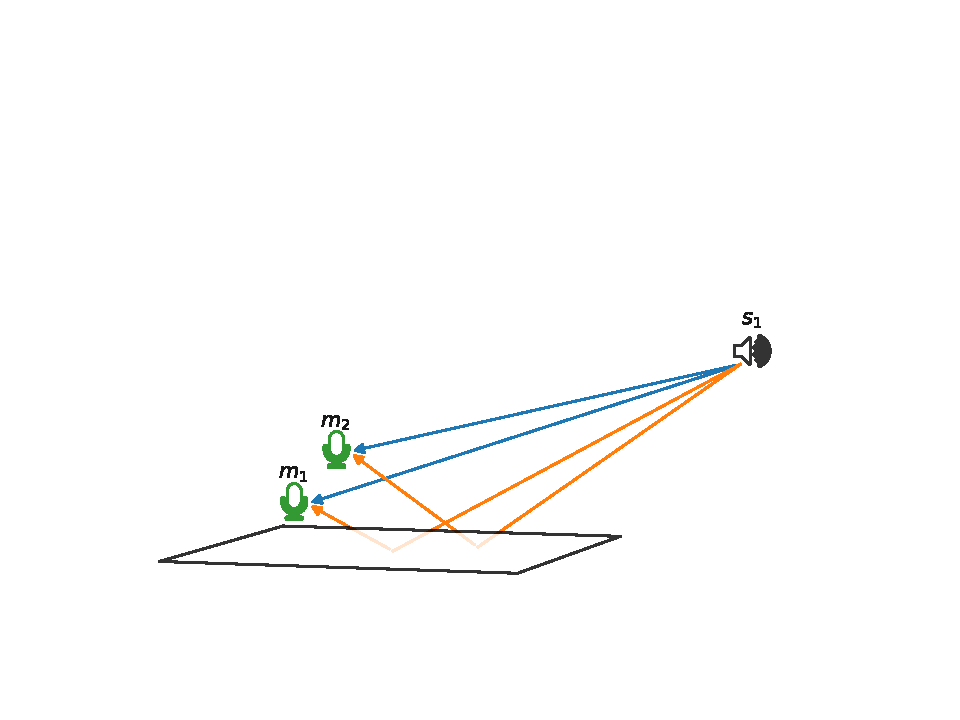
\includegraphics[trim={50 70 50 150},clip,width=\linewidth]{mirage/scene.pdf}
    \captionof{figure}{%
        Typical setup with one source source recorded by two microphones.
        The illustration shows direct sound path (blue lines) and resulting first-order echoes (orange lines).}
    \label{fig:lantern:scene}
}.
This is motivated by the application to \acf{SSL} that will be discussed in~\cref{ch:mirage}.
The reason why we consider only microphone-pair is that this approach can be generalize later to microphone array.
In fact, by considering all the pairs, it is possible to aggregate all their estimation in a second step using the knowledge about the array geometry.
Such an approach can be referred to the \ac{SRP-PHAT}~\citeonly{dibiase2001robust} algorithm used is \ac{SSL}.
In the remaining part of this chapter, we will discuss how to achieve robust first-echo estimation and how it could be generalized to multiple echoes.

\subsection{Simple Case: $\numEchs = 1$}
Our approach is to train a \ac{DNN} on a dataset simulating the considered close-surface scenario.
Under this assumption and the \acf{STFT} signal model presented in~\cref{eq:processing:stft}, we can consider the following simplified model for the \acfp{RTF},
\begin{equation}\label{eq:mirage:rir}
    \FLT_\idxMic[k] = \sum_{\idxEch=0}^{\numEchs=1}  \; \alpha_\idxMic^{(\idxEch)}[k] \; \cste^{- \csti 2 \pi f_k \tau_\idxMic^{(\idxEch)}} \; + \; \varepsilon_\idxMic[k],
\end{equation}
where $\tau_\idxMic^{(\idxEch)}$ and $\alpha_\idxMic^{(\idxEch)}[k]$ are the echoes's time of arrival and amplitude, respectively.
The $f_k$ denotes $k$-th frequency bin and the error term $\varepsilon_i[k]$ collects later echoes, the reverberation tail, diffusion, and noise.

\mynewline
We model the \AER/ problem as multi-target regression problem, namely the output on the model are multiple real-valued parameters.
Following the approaches suggested in~\citeonly{deleforge2015acoustic,gaultier2017vast}, we consider the instantaneous \acf{ILD} and the \ac{IPD} (see~\cref{eq:mirage:features} as input features.
As discussed in~\cref{subsec:processing:steering}, the \ac{ILD} and \ac{IPD} can be estimated from the \STFT/ of the microphone signals, such as,
\begin{equation} \label{eq:mirage:features}
\begin{cases}
    \ild[k]  =& \tfrac{1}{T} \sum_{l=1}^T \log{\abs{\frac{\MIC_2[k,l]}{\MIC_1[k,l]}}}, \\
    \ipd[k]  =& \tfrac{1}{T} \sum_{l=1}^T \frac{\MIC_2k,l]/ \abs{\MIC_2[k,l]}}{ \MIC_2k,l] / \abs{\MIC_1[k,l]}},\\
\end{cases}
\end{equation}
where $\MIC_i[k,l]$ is the \ac{STFT} of the $i$-th microphone.
\\More precisely, the input of the network is
\begin{equation*}
    \xi = \klist{ \ild, \kRe\set{\ipd}, \kIm\set{\ipd}}
    ,
\end{equation*}
namely the concatenation of the above features for all the frequencies.
Here $\kRe\set{\cdot}$ and $\kIm\set{\cdot}$ denote real and imaginary part operators, respectively.
Note that for the \ac{IPD}, the frequency $k=0$ is discarded because it is constant for every observation.

\mynewline
Initial investigation shown that learning directly the echoes arrival time and their amplitude yield huge estimation error, probable to the complexity of the task.
Motivated by the application in \ac{SSL} discussed in~\cref{ch:mirage}, we consider only the \acfp{TDOA} between the direct path propagation.
\begin{align}
    \tau_\mathtt{TDOA}  &= \tfrac{1}{c} \norm{\positionMicrophone_2 - \positionSource} - \tfrac{1}{c} \norm{\positionMicrophone_1 - \positionSource} = \tau_2^{(0)} - \tau_1^{(0)} \quad[\text{s}],\\
    \tau_\mathtt{iTDOA} &= \tfrac{1}{c} \norm{\mathring{\positionMicrophone}_2 - \positionSource} - \tfrac{1}{c} \norm{\mathring{\positionMicrophone}_1 - \positionSource} = \tau_2^{(1)} - \tau_1^{(1)} \quad[\text{s}],\\
    \tau_{\mathtt{TDOE},1}  &= \tfrac{1}{c} \norm{\mathring{\positionMicrophone}_1 - \positionSource} - \tfrac{1}{c} \norm{\positionMicrophone_1 - \positionSource} = \tau_1^{(1)} - \tau_1^{(0)} \quad[\text{s}],
\end{align}
where $\mathring{\positionMicrophone}_i$ denotes the position of the image of the microphone at position $\positionMicrophone_i$ with respect to the reflector.
Note that $\tau_{\mathtt{TDOE},2} = \tau_\mathtt{iTDOA} + \tau_{\mathtt{TDOE}, 1} - \tau_\mathtt{TDOA}$.
These three quantities are directly connected to \RIRs/, as illustrated in~\cref{fig:lantern:rirs_tdoa}\marginpar{%
\centering
\footnotesize
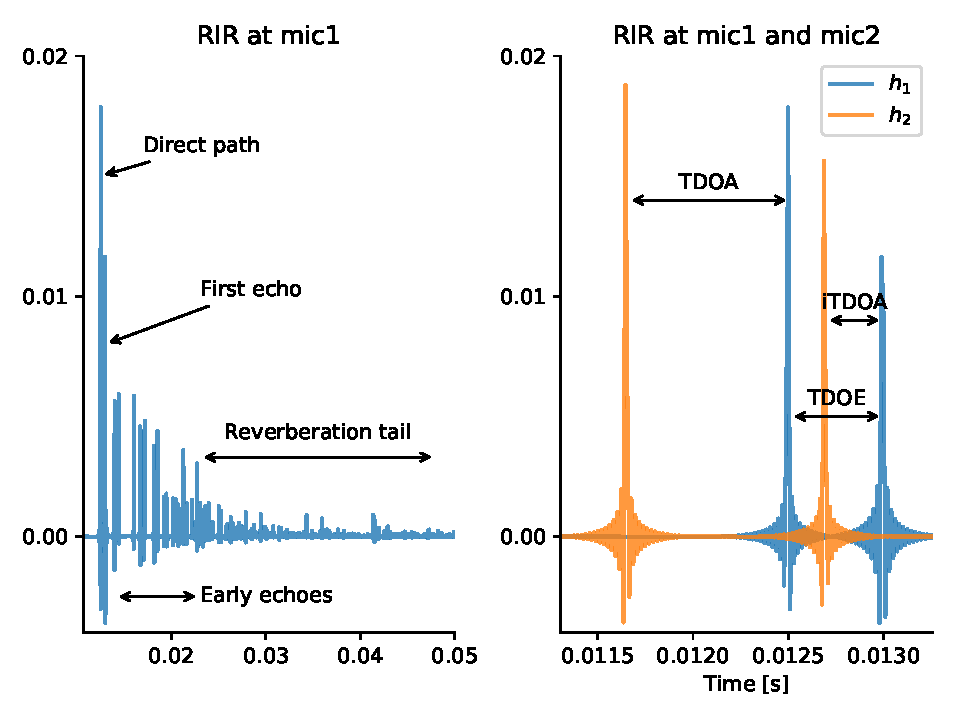
\includegraphics[trim={82mm 0 0 0},clip,width=\linewidth,height=7cm]{mirage/rirs.pdf}
\captionof{figure}{%
    Superposition of two \acp{RIR} and visualization of time difference of arrival between direct paths (\ac{TDOA}), first echoes (\ac{iTDOA}) and direct path and first echo (\ac{TDOE}).}
\label{fig:lantern:rirs_tdoa}
}. Let $V = \klist{\tau_{\mathtt{TDOA}}, \tau_{\mathtt{iTDOA}}, \tau_{\mathtt{TDOE},1}}\in\mathbb{R}^3$ be the vector of the parameters of interest
and $\calV = \set{\mathtt{TDOA}, \mathtt{iTDOA}, \mathtt{TDOE}_1}$ the set of corresponding labels.

\mynewline
In general, the mapping between $V$ and the proposed feature is not unique.
In particular, this happen when $\tau_2^{(\idxEch)} = \tau_1^{(\idxEch)}$ for $\idxEch=\set{0,1}$.
In order to avoid this, we preventively pruned all the entries with $| \tau_2^{(\idxEch)} - \tau_1^{(\idxEch)} | < 10^{-6}$ for $\idxEch=\set{0,1}$ from the dataset.


\newthought{As first investigation}, we used a simple \ac{MLP} architecture described in~\cref{subsec:lantern:mlp}.
This model consists of a $D$-dimensional input layer, a 3-dimensional output layer, and 3 fully connected hidden layers with respective input sizes $500$, $300$ and $50$.
\ac{ReLU} activation functions are used except at the output layer, and each hidden layer has a dropout probability $p_\text{do} = 0.3$ to prevent overfitting.
\\We use the mean square error loss function for training, that is,
\begin{equation}\label{eq:lantern:mlploss}
    \calL_\theta(V, \hat{V)} = \frac{1}{|\calV|} \sum_{b\in\calB} \sum_{v\in\calV} \powerOf{\tau_{v, b} - \hat{\tau}_{v, b}}
\end{equation}
where $e$ indexes one of \ac{TDOA} in $\calV$, $b$ indexes of an observation in the mini-batch $\calB$, and $\theta$ are the model parameters.

\mynewline
The \acf{nRMSE} is taken as validation metric\sidenote{
    The ac{nRMSE} takes values between $0$ (perfect fit) and $\infty$ (bad fit).
    If it is equal to $1$, then the prediction is no better than a constant.
    It is typically chosen because it is more robust to outliers than \ac{RMSE}.
} for assessing the quality of the estimation $\hat{V}$.
The network is manually tuned on a validation set to find the best combination of number of hidden layers, their sizes and $p_\text{do}$.

\mynewline{For training and validation} of the \ac{MLP} we generate many random, shoe-box room configurations using the software presented in \citeonly{schimmel2009fast}.
This software implements both the \acf{ISM} for simulating reflections and a ray-tracing algorithm for diffusion.
Room widths are uniformly drawn at random in $[3, 9]$ m, heights in $[2, 4]$ m.
Random source and microphones positions are used, respecting the close-surface scenario.\sidenote{
    A rejection-sampling strategies was used to approximate uniform distributions.
}
In particular, the microphones are at most 30~cm from the close-surface, placed 10~cm from each other,
and the absorption coefficients of the other walls are uniformly sampled in $(0.5, 1)$ and the one of the close-surface is in $(0, 0.5)$.
The same realistic diffusion profile \citeonly{gaultier2017vast} is used for all surfaces.
Around $90,000$ audio scenes are generated this way, yielding a \ac{RT$_{60}$} between $20$ ms and $250$ ms.
\\The \acp{RIR} are convolved with 1 sec of white-noise (wn) with no additional noise.
All signals and \acp{RIR} are sampled at $16$ kHz.
The \ac{STFT} is performed on $1024$ point with $50\%$ overlap.
Finally the features are computed as in~\eqref{eq:mirage:features} yielding a vector of size $D = 1534$ for each observation.
\\While we validate the \ac{MLP} on a portion of the dataset in a \textit{holdout} fashion, the test is conducted on 200 new \acp{RIR} convolved with both wn and speech (sp) utterances.
This set is generated similarly to the training and validation sets.
Moreover the test recordings are perturbed by external white noise at 10~dB \acf{SNR} (wn+n, sp+n).
The speech signals are normalized speech utterances of various lengths (from $1$ s to $6$ s), randomly selected from the TIMIT corpus.
% A free and open-source Matlab implementation of SRP-PHAT\footnote{\url{http://bass-db.gforge.inria.fr/bss_locate/}} is used to aggregate local angular spectra obtained from the DNN's output.
% The same toolbox is used for the implementation of SPR-PHAT with GCC-PHAT. For the latter method only real pairs are used.
% A sphere sampling with $\ang{0.5}$ resolution and coordinates $\theta \in [-179, 180]$ and $\phi \in [0, 90]$ is used for the DOA search.

\newthoughtpar{Experimental results}
To check the validity of \ac{TDOA} estimation with the \ac{MLP}, it is compared to a baseline algorithm \acf{GCC-PHAT} (see~\cref{subsec:mirage:1D-SSL}).
\ac{GCC-PHAT} is popular method for estimating \ac{TDOA} between two microphone recordings.
It is known to achieve good performance in case of broadband source signal and some robustness to noise level.
However, it was shown that as soon as the acoustic condition become challenging due to strong early echoes, high reverberation level and noise, the method performances decrease~\citeonly{chen2006time}.

\begin{table}[ht!]
    \begin{sidecaption}[Echo estimation with MIRAGE results]{%
        Normalize root mean squared error for TDOA estimation
    }[tab:lantern:tdoas-aoa]
    \centering
    \footnotesize
    \small
    \begin{tabular*}{\linewidth}{@{\extracolsep{\fill}}lcl|cccc@{}}
    \toprule
    &            &         &          & nRMSE           &\\
    &            & Input   &    \ac{TDOA}  	&   \ac{iTDOA} 		 &     \ac{TDOE}   	&\\
    \midrule
    & MIRAGE      &   wn    & 0.18    & 0.28  & 0.25 	& \\
    & MIRAGE      &   wn+n  & 0.68    & 0.69  & 0.89 	& \\
    & MIRAGE      &   sp    & 0.31    & 0.34  & 0.56    & \\
    & MIRAGE      &   sp+n  & 0.99    & 0.98  & 1.48 	& \\
    & GCC-PHAT    &   wn    & 0.21    & -     & -		& \\
    & GCC-PHAT    &   wn+n  & 0.68    & -     & -		& \\
    & GCC-PHAT    &   sp 	& 0.32    & -     & -		& \\
    & GCC-PHAT    &   sp+n  & 1.38    & -     & -		& \\
    \bottomrule
    \end{tabular*}
    \end{sidecaption}
\end{table}

\mynewline
\ac{TDOA} estimation errors using the proposed approach and \ac{GCC-PHAT} are presented in~\cref{tab:lantern:tdoas-aoa}.
Training a \ac{MPL} to estimate \acp{TDOA} brings similar performances as \ac{GCC-PHAT} in terms of nRMSE.
However, the estimation of \ac{iTDOA} and \ac{TDOE} seems to be a harder task for the such a simple \ac{MPL} model.
When some external noise is added, performance of both methods degrades.
This is a well-know and expected behavior for \ac{GCC-PHAT} and it suggests that noise should be considered also in the training phase. When
Nevertheless, our results confirm the possibility of retrieving early echoes from only two-microphone recordings.

\subsection{Robust learning-based TDOA estimation}
The above model was proposed in the our published work~\citeonly{di2019mirage}.
Later, more recent \ac{DNN} models were investigated, such as the \ac{CNN} proposed in \citeonly{nguyen2018autonomous} and similar to the one used in \citeonly{chakrabarty2017broadband} for the task of \ac{SSL}.

\begin{figure}[h]
    \begin{sidecaption}[CNN]{
        Architecture of the proposed deep neural network. Input and output dimensions for each stage are reported. The first dimension is the batch size $B = 200$.
    }[fig:lantern:cnn]
    \centering
    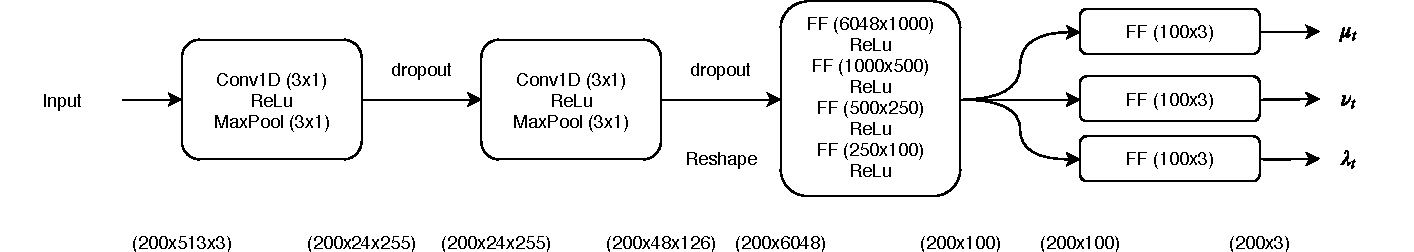
\includegraphics[width=\linewidth]{mirage/cnn.pdf}
    \end{sidecaption}
\end{figure}

\mynewline
As shown in~\cref{fig:lantern:cnn}, the architecture consists of two convolutional modules made of a one-dimensional convolutional layer (1DConv) followed by max-pooling along the frequencies, followed by \ac{ReLU} activation function and batch-normalization.
The second part consists of a cascade of fully connected feed-forward (FF) layers.
In order to perform 1D-convolution ond the right dimension, we re-arranged the input so that the each of features $\klist{ \ild, \kRe\set{\ipd}, \kIm\set{\ipd}}$ is considered as channel for the 1DConv.
After each layer a dropout probability $p_\text{do} = 0.3$ is applied.

\mynewline
In the \ac{MLP} model presented above in the previous section, the output consisted only in the \acp{TDOA} $V$.
However, to build a local angular spectrum, suitable for the \ac{SRP-PHAT}-like algorithm, both means and variances are needed.
Rather than identify these variances with the prediction errors, we explicitly modify the \ac{CNN} model to estimated them\sidenote{
    This idea is similar to the one proposed by Bishop in \ac{MDN} in \citeonly{bishop1994mixture}
    where the output of a neural network parametrizes a Gaussian mixture model.
}.
The main idea behind this design choice is that the learning model can assess its prediction quality.
This approach can be related to existing (Bayesian) data-fusion frameworks, but this direction wav not considered in this work.
\newcommand{\setTDOA}{\ensuremath{\set{\mathtt{TDOA}, \mathtt{iTDOA}, \mathtt{TDOE}}}}
\\To this end, we modify the output of the network to output mean and variances, namely
$V_{\calN} = \set{\mu_{\tau_t}, \sigma^2_{\tau_t}}$
for $t = \setTDOA$.
Moreover, we assume that conditional probability of observing the one of the \ac{TDOA} $\tau_t$ for $t \in \setTDOA$ given the observation $\xi$ in the batch $\Xi$, follows a Gaussian distribution, namely
\begin{equation}
    p(\tau_t \mid  \Xi ; \theta) \sim \calN\kparen{\mu_{\tau_t}(\xi_b;\theta), \sigma^2_{\tau_t}(\xi_b;\theta)}
\end{equation}
where the variance
and the the training loss function
 of~\cref{eq:mirage:mlploss}
\begin{equation}\label{subsec:mirage:mlpcost}
    \calL(V, \hat{V)} = \frac{1}{3} \sum_{b}  \powerOf{\tau_{\mathtt{TDOA}, b} - \hat{\tau}_{\mathtt{TDOA}, b}}
                                            + \powerOf{\tau_{\mathtt{iTDOA}, b} - \hat{\tau}_{\mathtt{iTDOA}, b}}
                                            + \powerOf{\tau_{\mathtt{TDOE}, b} - \hat{\tau}_{\mathtt{TDOE}, b}}
\end{equation}


\newthought{The proposed novel loss function} is the negative Student-T log-likelihood, which is implemented as follows:

\begin{equation}
\begin{split}
\mathcal{L}(\Theta) =& \sum_{x \in B} \sum_{t \in V}\ \dfrac{1}{2} \log (\nu_t\pi_t)
                        + \dfrac{1}{2} \log(\lambda_t^2)
                        - \log  \Gamma \left( \dfrac{\nu_t+1}{2} \right)\\
                    &    + \log  \Gamma \left( \dfrac{\nu_t}{2} \right)
                        + \dfrac{\nu_t+1}{2}
                        \log \left( 1  + \dfrac{\norm{\mu_t, x_i)}}{\nu_t \lambda_t^2} \right)\\
\end{split}
\end{equation}

where $\Theta$ are the CNN parameters and $\Gamma$ is the Gamma function. The summation over $i$ corresponds to the sum among of all the sample $x$ of the batch $B$. and the summation over $t$ corresponds to the sum among the three quantities in V (TDOA, iTDOA, TDOE). It follows that for each each input the network will return the parameters of 3 Student-T distribution ($\mu_t, \nu_t, \lambda_t$) for each variable $t = { \text{TDOA}, \text{iTDOA}, \text{TDOE} }$. Hereafter we denote with $V_{\mathcal{ST}}$ the set of the 9 network outputs.
We use the Adam optimizer ant the normalized root mean square error (nRMSE) is taken as validation metric (see Section~\ref{subsec:eval_synth_tdoa}). The network is manually tuned on a validation set to find the best combination of number of hidden layers and their sizes
Once an estimate $\hat{V_\mathcal{ST}}$ of the parameters of the 3 distribution is returned by the CNN, they are converted to synthetic local angular spectra and passed to an SRP-PHAT method together with the relative positions of true and image microphones which are assumed known. We call this algorithm MIRAGE. The synthetic local angular spectra consist of Student-t distribution with parameters $\mu, \nu$ and $\lambda$.
and $V \in \mathbb{R}^3$ as output parameters.


We use a simple fully-connected DNN architecture consisting of a $D$-dimensional input layer,
a $3$-dimensional output layer, and 3 fully connected hidden layers with respective input
sizes $500$, $300$ and $50$. Rectified linear unit (ReLU)
activation functions are used except at the output layer,
and each hidden layer has a dropout probability $p_\text{do} = 0.3$.
We use the mean square error loss function for training and the Adam optimizer \cite{kingma2014adam}.
The normalized root mean square error (nRMSE) is taken as validation
metric\footnote{The nRMSE takes values between $0$ (perfect fit) and $\infty$ (bad fit).
If it is equal to $1$, then the prediction is no better than a constant.}.
The network is manually tuned on a validation set to find the best combination of number of hidden layers, their sizes and $p_\text{do}$.
Once time delay estimates $\hat{V}$ are returned by the DNN, they are converted to synthetic
local angular spectra and passed to $\Psi_\text{SRP}$ (See Sec. \cref{subsec:mirage:2D-SSL})
together with the relative positions of true and image microphones which are assumed known.
We call this algorithm MIRAGE. The synthetic local angular spectra consist of Gaussians
centered at $\hat{V}$ and with variances equal to the prediction errors made by
the DNN on the validation set.

For training and validation, the RIRs are convolved with 1 sec of white-noise with additional noise with SNR in $(0,20)$ dB.
All signals and RIRs are sampled at $16$ kHz. The STFT is performed on $1024$ point with $50\%$ overlap. Finally the features are computed as in~\eqref{eq:features} yielding a vector of size $D = 1534$ for each observation.
While we validate the CNN on a portion of the dataset in a \textit{holdout} fashion, the test is conducted on 200 new RIRs convolved with both speech utterances.
This set is generated similarly to the training and validation sets. Moreover the recordings are perturbed by external white noise as in the training set. The speech signals are normalized speech utterances of various lengths (from $1$ s to $6$ s), randomly selected from the TIMIT corpus.
A re-implement version of SRP-PHAT is used to aggregate local angular spectra obtained from the DNN's output and as a baseline.
 However the original MATLAB code for SRP-PHAT can be found at \url{http://bass-db.gforge.inria.fr/bss_locate/}. A sphere sampling with $1$ degree resolution and coordinates $\theta \in [-179, 180]$ and $\phi \in [0, 90]$ degrees is used for the DOA search.


\section{Conclusion and perspective}

\newthought{Towards the case $\numEchs > 2$}

\newthought{Better features: \RTF/}

\newthought{Better architecture: Physical-based learning and unfolding}


% \begin{table}[ht!]
%     \begin{sidecaption}[Echo estimation with MIRAGE results]{%
%         Normalize root mean squared error for TDOA estimation and mean angular error in ${}^\circ$ (with accuracies ($\%$))
%         for AOA estimation with $\ang{10}$ and $\ang{20}$ angular tolerance.
%     }[tab:mirage:tdoas-aoa]
%     \centering
%     \footnotesize
%     %\scriptsize
%     \begin{tabular}{cl|ccc|cc}
%     \toprule
%                 &         &          & nRMSE        &                   &\multicolumn{2}{c}{ACCURACY}  \\
%                 & Input   &    \scriptsize{TDOA}  	&   \scriptsize{iTDOA} 		 &     \scriptsize{TDOE} 		 & $\theta<\ang{10}$ &  $\theta<\ang{20}$ \\
%     \midrule
%     MIRAGE      &   wn    & 0.18    & 0.28  & 0.25 	& 4.10 (77)	& 5.97 (97) \\
%     MIRAGE      &   wn+n  & 0.68    & 0.69  & 0.89 	& 5.00 (26)	& 9.89 (54) \\
%     MIRAGE      &   sp    & 0.31    & 0.34  & 0.56  & 4.83 (63)	& 7.26 (82) \\
%     MIRAGE      &   sp+n  & 0.99    & 0.98  & 1.48 	& 4.60 (16)	& 9.88 (35) \\
%     GCC-PHAT    &   wn    & 0.21    & -     & -		& 4.22 (81) & 6.19 (97) \\
%     GCC-PHAT    &   wn+n  & 0.68    & -     & -		& 4.03 (65) & 5.34 (83) \\
%     GCC-PHAT    &   sp 	  & 0.32    & -     & -		& 4.08 (82) & 5.34 (97) \\
%     GCC-PHAT    &   sp+n  & 1.38    & -     & -		& 4.70 (19) & 8.38 (32) \\
%     \bottomrule
%     \end{tabular}
%     \end{sidecaption}
% \end{table}